\begin{tikzpicture}
% comment it out at the end
%\draw[help lines] (0,0) grid(20,20);

% STS rectangle
\coordinate (TLSTS) at (4,16);
\coordinate (BRSTS) at (12,12) {};

% Draw rectangles and their names in corners
\draw [ultra thick, rounded corners, blue] (TLSTS) rectangle (BRSTS);
\node [below right] at (TLSTS) {Short Term Smoother};

% Draw Vision feeder
%\draw [ultra thick, rounded corners, blue] (TLDF) rectangle (BRDF);
%\node [below right] at (TLDF) {Data input};



% Draw data flow
\node (DF) at (2.5,13) {};
\draw [thick, ->] ($(DF) + (0,1.5)$) -- ($(TLSTS) - (0,1.5)$) node [above left] {Vision};
\draw [thick, ->] ($(DF) + (0,1)$) -- ($(TLSTS) - (0,2)$) node [above left] {IMU};
\draw [thick, ->] ($(DF) + (0,0.5)$) -- ($(TLSTS) - (0,2.5)$) node [above left] {GPS};
%\draw [thick, ->] ($(BRDF) + (0,0.5)$) -- ($(BRDF) + (1,0.5)$)
  %-- ($(BRDF) + (1,-5)$) --  ($(TLLTS) - (0,2)$)  node [above left] {GPS};


\node (DD) at (4,16) {};
\draw [thick, ->] ($(DD)+(1,-4)$) -- ($(DD)+(1,-6)$);
\draw [thick, ->] ($(DD)+(1.5,-4)$) -- ($(DD)+(1.5,-6)$);
\draw [thick, ->] ($(DD)+(2,-4)$) -- ($(DD)+(2,-6)$);
\draw [thick, ->] ($(DD)+(6,-6)$) -- ($(DD)+(6,-4)$);

\node [align=left, right] at (6,11) {Pose estimates\\Vision\\IMU};

%\draw [thick, ->] ($(TLLTS)+(6,0)$) -- ($(TLSTS)+(6,-4)$);
\node [align=left, right] at (10,11) {"fixed" \\landmark positions};

% node [right] {Pose estimates};

% TODO not a nice solution to include the pdf
\node at (8.5,14) {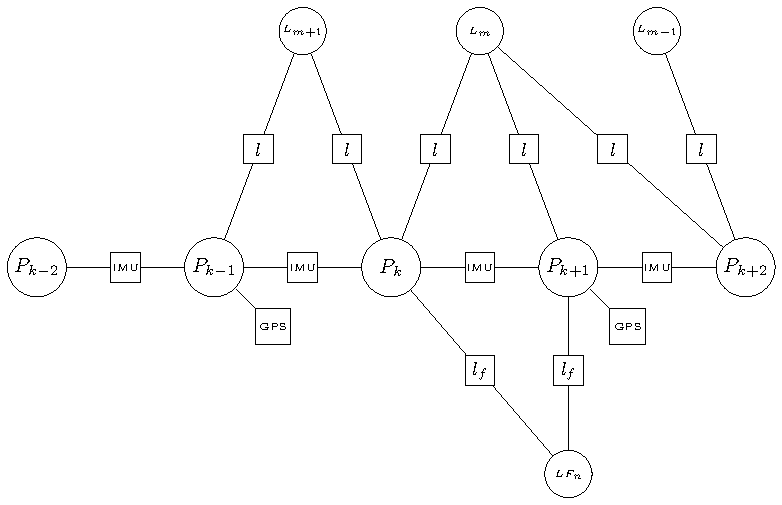
\includegraphics[scale=0.4]{./../factor_graph/factor_graph.pdf}};
%\node at (10,8) {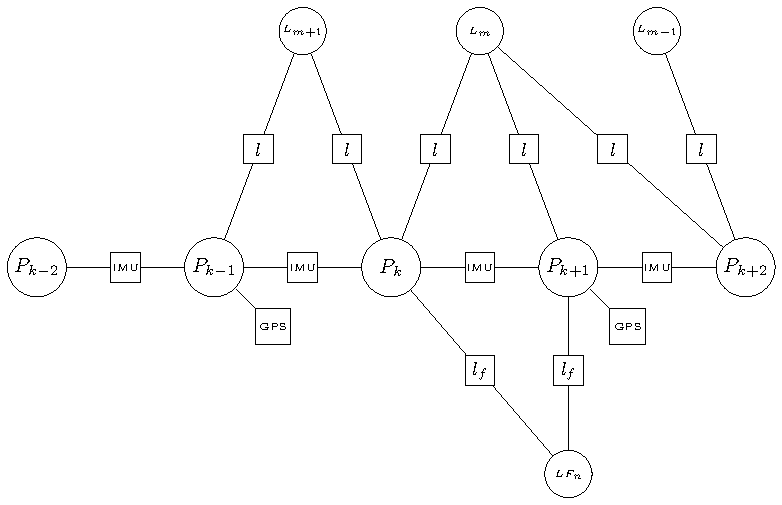
\includegraphics[scale=0.2]{./../factor_graph/factor_graph.pdf}};


%% TODO add it below \end
%\caption{Do not forget!
%Make it explicit enough that readers
%can figure out what you are doing.}

% \draw [ultra thick, rounded corners, purple] (5.5,8.5) ellipse (0.5 and 0.2);
% \node (v1) at (5,7.1) {};
% \node (v2) at (5,8.6) {};
% \node (v3) at (6,8.6) {};
% \node (v4) at (6,7.1) {};
% \draw [ultra thick, rounded corners, purple] (v1) edge (v2);
% \draw [ultra thick, rounded corners, purple] (5,7.25) arc (180:360:0.5 and 0.2);
% \draw [ultra thick, rounded corners, purple] (v3) edge (v4);
% 
% \draw [->](6.75,7.701) arc (-120.0007:-60:1.5);
% \draw [->](8.25,8.299) arc (59.9993:120:1.5);
% 
% \node at (5.5,7.75) {Map};
% 
% \node at (7.5,8) {Translator};


\end{tikzpicture}


    
    
    